\documentclass[11pt,a4paper]{article}

% ---------------------------------------------------------------------------
% Policy Store — Technical Architecture Document
% Single-column layout, intended for software-architecture writing:
% context, decisions, component views, interfaces, trade-offs.
% ---------------------------------------------------------------------------

\usepackage[margin=2.5cm]{geometry}
\usepackage{amsmath,amssymb}
\usepackage{microtype}
\usepackage{booktabs}
\usepackage{enumitem}
\usepackage{graphicx}
\usepackage{xcolor}
\usepackage{listings}
\usepackage{fancyhdr}
\usepackage[hidelinks]{hyperref}
\emergencystretch=3em

% --- Colors -----------------------------------------------------------------
\definecolor{codebg}{gray}{0.96}
\definecolor{codeframe}{gray}{0.75}
\definecolor{accent}{RGB}{40,60,110}

% --- Code / configuration snippets ------------------------------------------
\lstset{
  basicstyle=\ttfamily\small,
  backgroundcolor=\color{codebg},
  frame=single,
  rulecolor=\color{codeframe},
  framerule=0.3pt,
  breaklines=true,
  columns=fullflexible,
  keepspaces=true,
  showstringspaces=false,
  aboveskip=1em,
  belowskip=1em,
}

% --- Headers / footers -------------------------------------------------------
\pagestyle{fancy}
\fancyhf{}
\fancyhead[L]{\small\itshape Policy Store --- Architecture}
\fancyhead[R]{\small\itshape Draft 0.1}
\fancyfoot[C]{\small\thepage}
\renewcommand{\headrulewidth}{0.3pt}

% --- Convenience macros -------------------------------------------------------
\newcommand{\term}[1]{\emph{#1}}                 % first use of a defined term
\newcommand{\component}[1]{\textsf{#1}}          % architectural component name
\newcommand{\field}[1]{\texttt{#1}}              % field / attribute / API name

% Architecture Decision Record block
\newcounter{adr}
\newenvironment{decision}[1]{%
  \refstepcounter{adr}%
  \par\medskip\noindent
  \textbf{\color{accent}Decision \theadr\ --- #1}\par\nopagebreak\noindent
  \begingroup\small
}{%
  \endgroup\par\medskip
}

\title{\textbf{Policy Store}\\[0.3em]
\large Interoperability for Policy Organization, Persistence,\\
\large Exchange, and Evaluation}
\author{Nicola Gallo}
\date{16 July 2026}

\begin{document}
\maketitle
\thispagestyle{empty}

% --- Document control ---------------------------------------------------------
\begin{center}
\small
\begin{tabular}{@{}ll@{}}
\toprule
Status   & Draft \\
Version  & 0.1 \\
Scope    & Policy Store \\
\bottomrule
\end{tabular}
\end{center}

\begin{abstract}
\noindent
This document explains why interoperability is necessary for the
organization, persistence, exchange, and evaluation of authorization
policies. Policies are expressed in versioned languages,
evaluated by versioned runtimes, and often need to be co-located with the
decision point that evaluates them. Organizing, persisting, and transferring
them reliably --- including over constrained networks --- is therefore an
architectural requirement.
\end{abstract}

\tableofcontents
\newpage

% ------------------------------------------------------------------------------
\section{Context and Problem Statement}

Policies are, first of all, languages. Like any language, a policy language
is expressive within the context it was designed for; no single language
fits every domain, and this is precisely why different types of policy
languages exist.

A policy language is evaluated by a runtime. Runtimes are versioned, and
policy languages themselves potentially evolve through versions as well:
a policy can only be evaluated by a runtime that supports the version of
the language the policy is written in. Language version and runtime version
must therefore be matched explicitly.

Furthermore, there are different types of policies --- not only application
policies, as discussed later in this document. Policies often need to be
co-located with the decision maker, the Policy Decision Point (PDP). This
requires a way to transfer policies efficiently, suitable for low-bandwidth
links as well, and protected so that an interrupted transfer can be resumed
safely.

For these reasons, policies must be organized, persisted, and made
transferable and understandable across systems: this is the interoperability
problem this document addresses.

% ------------------------------------------------------------------------------
\section{Policy Language and Runtime Structure}

\subsection{Policies as Objects}

A policy must be treated, first of all, as an \term{object} --- not as a
file. A file carries no guarantees about its own meaning: its
interpretation depends on where it happens to be placed, on naming
conventions, and on the tooling that reads it. An object, by contrast, is
self-describing. To be exchanged between systems, a policy object must
carry at least the following properties:

\begin{itemize}[nosep]
  \item a stable, unique \term{identifier}, so that the policy is
        addressable independently of any storage layout;
  \item the \term{language} it is written in and the \term{language
        version} it targets;
  \item its \term{type} (for example, a policy proper versus the schema
        the policies are written against);
  \item its \term{content}, in a form the declared runtime can evaluate.
\end{itemize}

Identity and meaning are intrinsic to the object: they travel with it,
they do not derive from its position in a directory tree.

\subsection{Logical Grouping}

For the same reason, policies are not grouped as filesystem trees but as
\term{logical groups}. A group collects the policies that are meant to be
managed and evaluated together. The filesystem layout used while
authoring is an editing convenience; it is not the semantic structure of
the group, and it must not be what a decision point relies on. Within a
group, policies are organized under logical \term{paths} (partitions),
and each partition declares its own characteristics --- language, schema,
runtime. A group is therefore potentially \term{multi-language}: policies
under different paths may be written in different languages and evaluated
by different runtimes, while still being organized, versioned, and
transferred as a single unit.

\subsection{The Manifest}

Every group must therefore include a \term{manifest}: a declaration that
states, for each logical path, what type of policies it contains, in
which language and language version they are expressed, and which runtime
--- at which version --- is able to evaluate them. The manifest is what
allows a consumer, a PDP in particular, to decide \emph{before} loading
the group whether it can evaluate it at all, resolving the
language-version/runtime-version matching problem stated in the previous
section. A non-normative pseudo-JSON manifest:

\begin{lstlisting}
{
  "metadata": {
    "name": "commerce-authz",
    "description": "Authorization model for the commerce domain"
  },
  "runtimes": {
    "cedar-stable": {
      "language": { "name": "cedar", "version": ">=4.0.0" },
      "engine":   { "name": "sample-engine", "version": ">=1.2.0" }
    },
    "rego-stable": {
      "language": { "name": "rego", "version": ">=1.0.0" },
      "engine":   { "name": "other-engine", "version": ">=0.60.0" }
    }
  },
  "partitions": {
    "/":       { "runtime": "cedar-stable", "schema": true },
    "/agents": { "runtime": "cedar-stable", "schema": false },
    "/infra":  { "runtime": "rego-stable",  "schema": false }
  }
}
\end{lstlisting}

The structure captures the three concerns separately. The
\field{runtimes} section declares one or more evaluation environments:
each entry binds a language and a version range to an engine and its
version range, so compatibility is expressed as explicit constraints
rather than assumed. The \field{partitions} section maps every logical
path of the group to one declared runtime and states whether that path
carries a schema. Because each partition binds to its own runtime, a
single group can mix policy languages without ambiguity: a consumer
knows, path by path, what it must be able to evaluate. Every partition
must reference a declared runtime, and a root partition must exist: the
manifest is validatable on its own, and the group is rejected as a whole
when the declaration is inconsistent.

Because the manifest is itself an object of the group, the group is
self-describing: it can be validated, versioned, and transferred as a
single coherent unit --- a property the rest of this document builds
upon.

% ------------------------------------------------------------------------------
\section{Policy Types}

Authorization is usually discussed as if application policies were the
whole story. Looking at an execution end to end, however, three distinct
types of policies emerge. To see why, we first need a minimal model of
what an execution is.

\subsection{The Canonical Execution Model}

An execution is nothing more than a \term{transaction initiated by a
root}: a principal expresses an intent, and that intent is carried out by
a chain of executors. At any point of the chain there is a previous
executor ($n-1$), a current executor ($n$), and a next executor ($n+1$):
the execution passes from $n-1$ through $n$ to reach $n+1$, always as a
consequence of the request that started at the root
(Figure~\ref{fig:canonical-execution}). The chain is not instantaneous,
either: a message sent at time $x$ may be handled by a workload
provisioned only at time $x+y$ --- the executors need not all exist at
the same time.

\begin{figure}[ht]
  \centering
  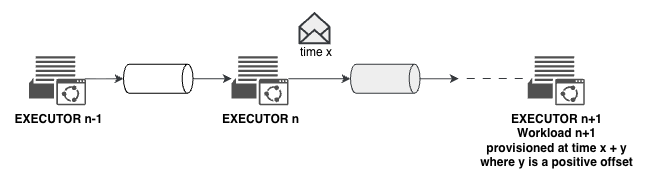
\includegraphics[width=\textwidth]{images/canonical-execution-model.png}
  \caption{The canonical execution model: a request initiated at the root
  flows through a chain of executors. The workload serving executor $n+1$
  may be provisioned after the message was sent.}
  \label{fig:canonical-execution}
\end{figure}

Each policy type governs a different point of this picture.

\subsection{Execution Policies}

\term{Execution policies} govern the execution chain itself: whether and
how step $n$ may reach step $n+1$, across which paths, under which
conditions. They do not answer application questions; they shape the way
the transaction is allowed to move.

Consider a security team analyzing a network. Starting from a single
request initiated at the root --- carrying a single token --- the team
wants to segment the network (micro-segmentation) and insert policies
along the execution paths. Those policies talk about segments, flows, and
protocols, not about business entities:

\begin{lstlisting}
# Execution policy (pseudo-code): micro-segmentation
permit execution-flow
  from  segment "scanners"
  to    segment "db-tier"
  when  origin.request == "sec-team/network-scan"
    and origin.token.scope contains "network:scan"
    and protocol == "tcp/5432"

deny execution-flow otherwise
\end{lstlisting}

\subsection{Semantic Translation Policies}

Executor $n$ may live in domain $A$ while executor $n+1$ lives in domain
$B$, and the two domains generally do not share the same vocabulary. When
the execution crosses the boundary, the authority expressed in the terms
of $A$ must be translated into the terms of $B$: this is the job of
\term{semantic translation policies}.

For example, a domain that models contracts may express an authority as
\field{ACCEPT-CONTRACT}; the receiving domain has no such concept, and
the closest equivalent requires two of its own privileges:

\begin{lstlisting}
# Translation policy (pseudo-code): domain A -> domain B
translate authority "contract:accept"        # vocabulary of A
     into "user:accept" and "admin:accept"   # vocabulary of B
\end{lstlisting}

A translation must be meaning-preserving and, crucially, non-expansive:
what the translated authority permits in $B$ must not exceed what the
original authority permitted in $A$.

\subsection{Application Policies}

When the execution finally reaches the application, \term{application
policies} evaluate the request in business terms: may this subject
perform this action on this resource, given the schema and the context.
This is the policy type most authorization systems focus on --- necessary,
but only one of the three.

\subsection{The Limits of the Subject-Centric Model}

Most authorization systems and APIs in use today are built around a
single request shape: \emph{may subject $S$ perform action $A$ on
resource $R$ in context $C$?} That shape is inherited from the world in
which authorization lived entirely inside one application, and it
captures application policies well --- and nothing else. Execution
policies do not speak about subjects and resources: they speak about
steps, paths, and flows. Translation policies do not answer an access
question at all: they map authority between vocabularies.

Forcing everything into the subject-centric shape leads to awkward
questions. If a translation policy must be evaluated when the execution
crosses a domain boundary, what evaluates it --- a second, ad hoc
decision point? If an execution policy must be validated inside the
network path, does the network now host an application-style PDP? A model
whose only primitive is the subject tuple leaves every other policy type
either squeezed into that mold or outside governance entirely. Both the
store and the evaluation model must be aware of policy types.

\subsection{The Non-Expansion Invariant}

The root has an \term{origin}: the authority selected when the intent was
expressed. Whatever the policies decide --- execution, translation, or
application --- the execution must never end up holding more authority
than that origin. This invariant applies to \emph{all} policy types.

The risk is concrete because policies are chained along the execution:
governance effects and application effects concatenate step after step.
Suppose one policy in the chain permits more than necessary. If its
result is simply accepted, the execution acquires authority it never
received from its origin. The rule must therefore be that at every step
the effective authority is the \emph{intersection} of what the policies
grant with the authority the step received at entry:
\[
A_{\mathit{effective}} \;=\; A_{\mathit{granted}} \,\cap\, A_{\mathit{entry}}
\]
Anything a policy grants beyond the entry authority is clipped;
otherwise, authority expands.

Figure~\ref{fig:expansion-bug} shows how an expansion can look perfectly
legitimate. Two independent executions (\emph{lineages}) run through the
same infrastructure: each one, taken alone, only ever attenuates its
authority. A defect then composes authority \emph{across} the lineages,
and the final executor of lineage 1 ends up holding \field{read all} ---
a privilege its own origin never granted, since it started from
\field{read foo}. Every step looked locally valid; the resulting security
state is not.

\begin{figure}[ht]
  \centering
  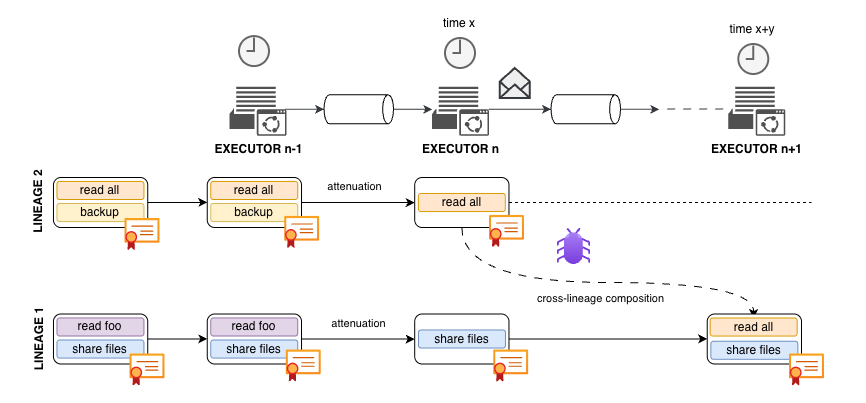
\includegraphics[width=\textwidth]{images/bug-valid-security-state.png}
  \caption{Authority expansion through cross-lineage composition: each
  lineage only attenuates its own authority, yet a defect merges
  authority across lineages and the final step holds more than its origin
  ever granted.}
  \label{fig:expansion-bug}
\end{figure}

\subsection{Grouping by Policy Type}

The three types answer different questions, are evaluated at different
points of the chain, and are best expressed in different languages: a
language designed for network flows is a poor fit for business rules, and
vice versa. This is exactly why the manifest of the previous section must
allow a group to be organized \emph{per policy type}, with each partition
free to declare its own language and runtime:

\begin{lstlisting}
"partitions": {
  "/execution":   { "runtime": "netlang-stable", "schema": false },
  "/translation": { "runtime": "maplang-stable", "schema": false },
  "/app":         { "runtime": "cedar-stable",   "schema": true  }
}
\end{lstlisting}

\noindent\textbf{Note.} \field{netlang-stable} and \field{maplang-stable}
are deliberately fictional names: this is an example only, and no
specific language is implied. Execution and translation policies may be
expressed in an existing policy language (such as Rego or a JSON-based
DSL) or in a purpose-built custom language --- the model does not
prescribe which language fills which role; it only requires that each
partition declares its own.

One group, one coherent unit of governance --- several policy types, each
in the language that fits it best.

% ------------------------------------------------------------------------------
\section{Transferability and Persistence}

Exchanging policies as described so far imposes a set of properties on
how they travel and how they are stored. These properties are independent
of any specific storage or network technology.

\subsection{Transfer Only What Changes}

Policy distribution must work over low-bandwidth links, so exchange must
happen only when necessary and must carry only what is necessary. If one
policy changed out of ten thousand, only that one travels --- never the
whole group. This requires being able to tell \emph{what} changed without
comparing contents byte by byte, which is a consequence of how objects
are identified, as discussed next.

\subsection{Immutable, Verifiable Objects}

Every object is \term{immutable}: a change never modifies an object, it
produces a new one. And every object is \term{verifiable}: the receiver
must be able to check, from the object alone, that its content was not
altered in transit or at rest.

Both properties follow from \term{content
addressing}\footnote{\url{https://docs.ipfs.tech/concepts/content-addressing/}}:
the identifier of an object is derived from its content itself. Such an
identifier is unique \emph{across} systems --- two independent parties
compute the same identifier for the same content, with no registry or
coordination --- and verification reduces to recomputing it. Identical
content is also recognized as identical everywhere, which is exactly what
makes minimal transfer possible: two sides can agree on what the other is
missing by exchanging identifiers, not contents.

\subsection{Everything Is a Transferable Object}

With identity settled, the picture becomes uniform: policies, schemas,
manifests, and the groups that contain them are all objects. A group is
transferred as a set of objects and \term{recomposed} at the destination
by following identifiers. If a transfer is interrupted, it can resume
safely: objects already received are immutable and verifiable, so storing
them again is harmless and nothing needs to be re-negotiated from
scratch.

\subsection{Minimal Persistence}

Persistence must require nothing more than an associative map from
identifier to bytes. A directory on disk, an object store such as S3, or
an in-memory dictionary are all sufficient backends: no database schema,
no query engine, no storage-specific format. This keeps the model
deployable everywhere the policies need to go --- from cloud services to
edge nodes.

\subsection{Versioning and Auditing}

Finally, the history of a group must be first-class: every change
produces a new version, previous versions remain reconstructible, and it
must always be possible to answer \emph{which policies were in force at a
given point} --- a governance and auditing requirement, not a
convenience.

% ------------------------------------------------------------------------------
\section{The Ledger: A Git-like Structure}

The properties of the previous section --- content-addressed immutable
objects, delta transfer, key-value persistence, versioned history --- do
not need to be invented. A battle-tested system built exactly on them has
existed for two decades: Git.

Git as-is, however, is not the answer. It carries far more than needed
(working trees, branching and merging workflows, hooks); it is a
general-purpose content tracker, so it enforces no structure --- anything
can be committed, and nothing guarantees the invariants of a policy group
(a manifest, partitions, one policy per object); and it is not designed
for the evaluation path, where a decision point must materialize a
precise version of a group quickly, at every decision. The solution is
therefore a \term{git-like} object model, specialized and optimized for
policies: battle-tested ideas, without reinventing the wheel and without
inheriting what does not serve. We call the resulting structure a
\term{ledger}.

\subsection{Structure}

A ledger is an append-only, content-addressed history of one policy
group, built from three kinds of objects:

\begin{itemize}[nosep]
  \item a \term{blob} is a leaf object: a policy, a schema, or the
        manifest;
  \item a \term{tree} represents one partition of the group: the list of
        its entries, each with its name, type, and language metadata;
  \item a \term{commit} represents one version of the whole group: it
        references the manifest blob, one tree per partition, and the
        predecessor commit.
\end{itemize}

Every object is serialized in a canonical form and identified by the
content-derived identifier of its bytes; the ledger itself is just a
\term{ref}: a pointer to the head commit.

\begin{lstlisting}
commit #C2
  predecessor  -> commit #C1
  manifest     -> blob #M
  /execution   -> tree #T1 -> blob #P1, blob #P2
  /app         -> tree #T2 -> blob #P3, blob #S (schema)
\end{lstlisting}

\subsection{Why This Solves the Problem}

Each requirement stated in this document maps directly onto the ledger:

\begin{itemize}[nosep]
  \item \textbf{Structure by construction.} A commit must reference a
        valid manifest, and its trees mirror the declared partitions: a
        malformed group is rejected at the object level, not by
        convention.
  \item \textbf{Minimal transfer.} Unchanged content keeps the same
        identifier, so unchanged partitions share their trees and blobs
        across versions. Synchronizing two ledgers reduces to comparing
        refs, computing the missing commits, and transferring only the
        objects that the other side does not already have --- the
        one-changed-file-in-ten-thousand case transfers one blob, one or
        two trees, and one commit.
  \item \textbf{Resumable, low-bandwidth exchange.} Objects are verified
        on receipt by recomputing their identifier, and storing an object
        twice is idempotent: an interrupted synchronization resumes where
        it stopped.
  \item \textbf{Minimal persistence.} All objects, whatever their kind,
        live in any identifier-to-bytes store.
  \item \textbf{Versioning and auditing.} The predecessor chain is the
        complete history: any past version of the group can be
        reconstructed exactly, and a decision can be tied to the precise
        commit it was evaluated against.
  \item \textbf{Evaluation-friendly.} A decision point materializes one
        commit --- manifest, trees, blobs --- directly from the store,
        with no working tree and no checkout.
\end{itemize}

\subsection{A Runtime, Not a Bundle}

The obvious way to distribute policies --- and the wrong one --- is a
compressed archive: zip the files, ship the bundle to the decision point,
unpack, load. A bundle reintroduces everything the object model left
behind: filesystem semantics instead of self-describing objects,
whole-store transfer instead of deltas, no per-object verification, no
resumable exchange, and no history at the destination. It treats policies
as static configuration to be installed.

Policies are languages, as stated at the outset --- and at the point of
decision they behave like code: they are brought onto the consumer and
executed locally, as if they were libraries loaded into the process. What
sits at the consumer is therefore not an unpacker of bundles but a
\term{runtime}: a component that synchronizes its local ledger with the
policy store and evaluates the synchronized version in place, exactly as
a language runtime loads and runs a versioned library.

This is most visible at the edge. A device on an intermittent,
low-bandwidth link cannot re-download an archive at every change: it must
\term{synchronize}. It aligns its local ledger when connectivity allows
--- transferring only the missing objects, resuming where it stopped ---
and keeps deciding locally against the last verified commit even while
disconnected.

Interoperability, then, does not stop at the store format: it extends to
the runtime. Any conforming runtime must be able to synchronize any
conforming ledger, read its manifest, and evaluate the partitions whose
declared languages it supports --- so that the same policy group yields
the same decisions in the cloud, in a sidecar, or on a device.

\end{document}
